\documentclass[10pt]{article}

\usepackage{tabularx}
\usepackage[a4paper,margin=2.5cm, bottom=2.5cm]{geometry}
\usepackage{fancyhdr}
\usepackage{listings}
\usepackage{booktabs}
\usepackage{float}
\usepackage{subcaption}
% \usepackage{caption}
% \captionsetup{font=footnotesize}
\usepackage{graphicx}
\usepackage{amsmath}
\usepackage{amssymb}
\usepackage{amsthm}
\usepackage{array}
\usepackage[table]{xcolor}
\usepackage{pgfplots}
\pgfplotsset{compat=1.17}
\usepackage{pgfplotstable}
\usepackage{multirow}
\usepackage{tikz}
\usepackage[hidelinks]{hyperref}
\usepackage{titling}
\usepackage[polish]{babel} % Polish language support

\setlength{\headheight}{40pt}
\setlength{\parindent}{0pt}
\setlength{\parskip}{1ex}
\renewcommand{\headrulewidth}{0pt}

\pagestyle{fancy}
\fancyhead{}
\fancyhead[L]{
    \renewcommand{\arraystretch}{1.5}
    \begin{tabularx}{\textwidth}{|X|X|}
        \hline
        \bfseries Obliczenia inteligentne & \bfseries \thetitle \\
        \hline
    \end{tabularx}
}
\fancyfoot[C]{\thepage}

\renewcommand{\maketitle}{
    \thispagestyle{plain}
    \renewcommand{\arraystretch}{2}
    \vspace*{-8em}
    \footnotesize
    \begin{flushleft}
        \begin{tabularx}{\textwidth}{|X|X|}
            \hline
            \bfseries Obliczenia Inteligentne  & \bfseries \thetitle                           \\ \hline
            \multicolumn{2}{|l|}{
                \begin{tabular}[t]{@{}ll@{}} 
                    \textbf{Grupa:} Grupa 1
                    \hspace{4.5em}
                    \textbf{Dzień i czas:} Czwartek, 10:00
                    \hspace{4.5em}
                    \textbf{Rok akademicki:} 2023/24
                \end{tabular}
            } \\ \hline
            \multicolumn{2}{|l|}{
                \begin{tabular}[t]{@{}l@{\hspace{10em}}l@{}} 
                    \textbf{Imię i nazwisko:} \textsc{Jakub Pawlak} & \textbf{Imię i nazwisko:} \textsc{Magdalena Paku\l a} 
                \end{tabular}
            } \\
            \hline
        \end{tabularx}
    \end{flushleft}
    \renewcommand{\arraystretch}{1}
}


\usepackage{wrapfig}
\usepackage{multicol}
\usepackage{gensymb}
\usepackage{textcomp}

\title{Projekt 2 --- Zadanie 2}

% Not needed for page size A3
% \captionsetup{font=small}

\newcommand{\plotAccuraciesFromLoggedMetrics}[1]{
    \begin{tikzpicture}
        \begin{axis}[
            width=\linewidth,
            height=.5\linewidth,
            legend pos = south east,
            grid = major,
            legend style={font=\tiny},
            style = {font=\small},
            xmin=0,
            enlarge x limits = 0.05 ,
            ymin=0, ymax=1.05
        ]
            \addplot+[mark=none] table[x = epoch, y = train_acc] {#1};
            \addlegendentry{Train acc};

            \addplot+[mark=none, orange] table[x = epoch, y = val_acc] {#1};
            \addlegendentry{Test acc};
        \end{axis}
    \end{tikzpicture}
}

\geometry{a3paper}
\begin{document}

\maketitle
\normalsize

\section{Eksperyment 1: Architektury sieci splotowej dla MNIST (JakubPawlak)}\label{sec:ex1-pawlak_mnist}

\subsection*{Pierwsza architektura}

Pierwsza architektura składa się z warstwy splotowej z jądrem $5\times5$, na wyjściu której obraz ma 6 kanałów, następnie jest przepuszczony przez funkcję sigmoid oraz max pooling.
Zamierzeniem jest, aby ta warstwa wykrywała krawędzie lub rogi cyfr.
Z tego też powodu, użyto funkcji aktywacji sigmoid, ponieważ funkcja ReLU całkowicie zeruje ujemne wartości.
W przypadku wykrywania krawędzi, ujemne wartości mogą być używane do reprezentacji kierunku.

Drugi splot prowadzi do 16 kanałów i ponownie jest używana funkcja sigmoid oraz max pooling.
Zadaniem tej warstwy jest rozpoznanie większych, bardziej złożonych kształtów.
Finalnie ekstraktor prowadzi do tensora $16 \times 5 \times 5$, który zostaje spłaszczony.

Klasyfikator to MLP z rozmiarami warstw odpowiednio $400,120,84,10$, używający sigmoidy jako funkcji aktywacji.

\pgfplotstableread[col sep=comma]{data/kuba/mnist/large.csv}\kubaMnistLarge{}

\begin{figure}[H]\centering
    \begin{subfigure}[t]{.55\textwidth}
        \plotAccuraciesFromLoggedMetrics{\kubaMnistLarge}
        \caption{Wykres zmian accuracy}
    \end{subfigure}
    \hspace{2em}
    \begin{subfigure}[t]{.34\textwidth}
        \centering
        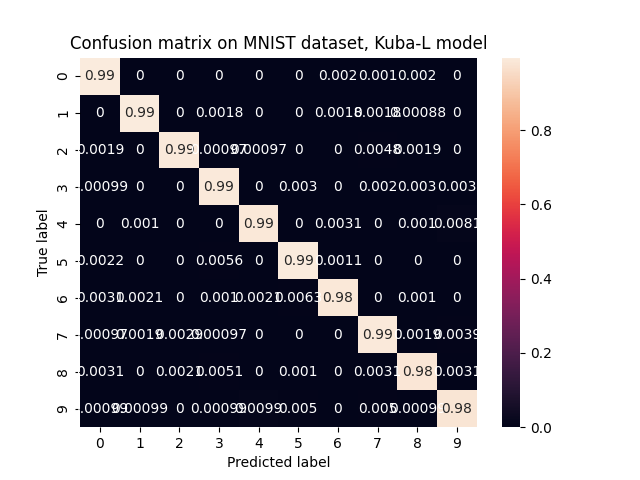
\includegraphics[width=\linewidth]{img/kuba/mnist/large_cm.png}
        \caption{Macierz pomyłek}
    \end{subfigure}
    \caption{Wyniki dla 1 architektury (Train acc: 0.997; Test acc: 0.987)}
    \label{fig:exp1_kuba_mnist}
\end{figure}


\subsection*{Druga architektura, prowadząca do ekstrakcji 2 cech}


\pgfplotstableread[col sep=comma]{data/kuba/mnist/smol.csv}\kubaMnistSmol{}

\begin{figure}[H]\centering
    \begin{subfigure}[t]{.55\textwidth}
        \plotAccuraciesFromLoggedMetrics{\kubaMnistSmol}
        \caption{Wykres zmian accuracy}
    \end{subfigure}
    \hspace{2em}
    \begin{subfigure}[t]{.34\textwidth}
        \centering
        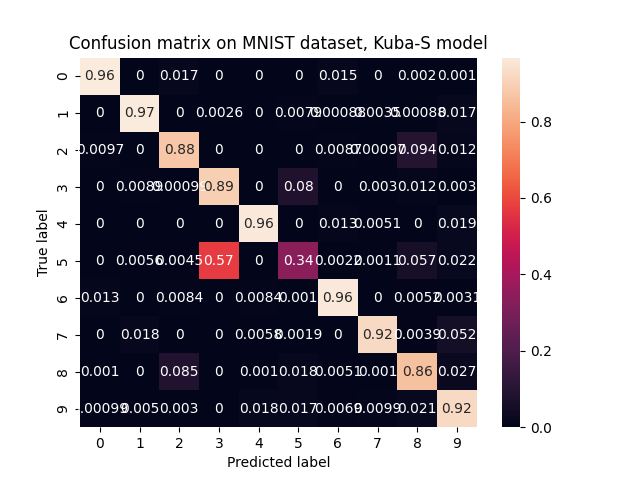
\includegraphics[width=\linewidth]{img/kuba/mnist/smol_cm.png}
        \caption{Macierz pomyłek}
    \end{subfigure}
    \caption{Wyniki dla 2 architektury (Train acc: 0.836;Test acc: 0.866)}\label{fig:kuba/mnist/smol}
\end{figure}

\begin{wrapfigure}[12]{r}{0.4\textwidth}
    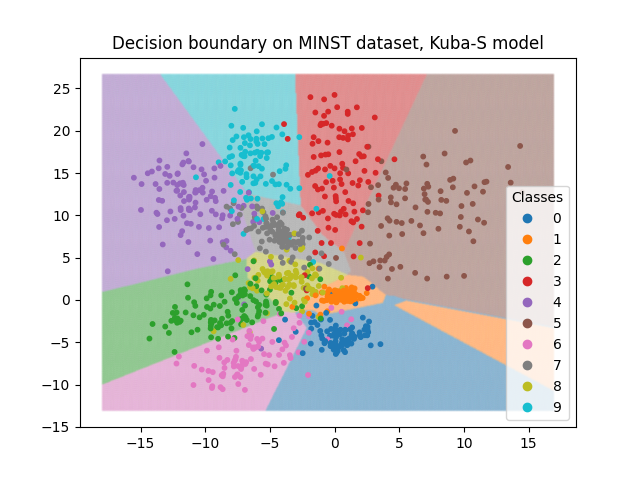
\includegraphics[width=\linewidth]{img/kuba/mnist/smol_db.png}
    \caption{Granica decyzyjna dla arch.~2}\label{fig:kuba/mnist/smol/decision_boundary}
\end{wrapfigure}

W drugiej architekturze warunkiem koniecznym jest rozmiar wektora cech, wynoszący 2 cechy.
Jest to umotywowane chęcią stworzenia wizualizacji granic decyzyjnych.
Ekstraktor cech składa się z następujących warstw:
\tiny
\begin{verbatim}
(feature_extractor): Sequential(
    (0): Conv2d(1, 10, kernel_size=(5, 5), stride=(1, 1), padding=(2, 2))
    (1): ReLU()
    (2): Dropout2d(p=0.1, inplace=False)
    (3): MaxPool2d(kernel_size=2, stride=2, padding=0, dilation=1, ceil_mode=False)
    (4): Conv2d(10, 5, kernel_size=(5, 5), stride=(1, 1))
    (5): ReLU()
    (6): MaxPool2d(kernel_size=2, stride=2, padding=0, dilation=1, ceil_mode=False)
    (7): Conv2d(5, 2, kernel_size=(3, 3), stride=(1, 1))
    (8): ReLU()
    (9): Flatten(start_dim=1, end_dim=-1)
    (10): Linear(in_features=18, out_features=2, bias=True)
)
(classifier): Sequential(
    (0): Linear(in_features=2, out_features=5, bias=True)
    (1): ReLU()
    (2): Linear(in_features=5, out_features=10, bias=True)
)
\end{verbatim}
\normalsize

W tym modelu, aby jeszcze bardziej zmniejszyć ilość cech, zastosowano jeszcze jedną warstwę konwolucyjną.
Finalnie, ekstraktor cech zawiera jedną w pełni połączoną warstwę, w celu redukcji do 2 cech.

W tym modelu postanowiono również przeprowadzić eksperyment z użyciem warstwy dropout w celu poprawienia
odporności na overfitting.
Pomimo, że z racji na dużą liczność zbioru treningowego, w eksperymencie 1 nie ma dużego ryzyka przetrenowania,
sytuacja może ulec zmianie w eksperymencie 2. Negatywnym efektem użycia warstwy dropout jest spowolnienie procesu uczenia, co jest dobrze widoczne na wykresie.

Warstwy konwolucyjne prowadzą do finalnego tensora o wymiarach $2 \times 3 \times 3$, 10więc na końcu ekstraktora cech znajduje się jeszce jenda warstwa linear, tworząca 2-wymiarowy wektor cech.

Klasyfikator zawiera jedną warstwę ukrytą o rozmiarze 5 neuronów, z funkcją relu, a następnie warstwę wyjściową o rozmiarze 10 neuronów.

\pagebreak
\section{Eksperyment 1: Architektury sieci splotowej dla MNIST (Magdalena Pakuła)}\label{sec:ex1-pakula_mnist}

\subsection*{Pierwsza architektura}
Zawiera trzy warstwy splotowe każda warstwa wydobywa coraz bardziej abstrakcyjne cechy. Warstwy początkowe rejestrują krawędzie i tekstury, podczas gdy warstwy głębsze rejestrują kształty i bardziej złożone wzory. Ma to kluczowe znaczenie w przypadku rozpoznawania cyfr, gdzie należy rozróżnić subtelne różnice.
Po każdej wartwie splotowej następuje redukcja wymiarowości, dzięki użyciu MaxPool2d, co pozwala sieci skupić się na najbardziej istotnych cechach cyfr, poprawiając generalizację.
Stopniowy wzrost filtrów (8, 16, 32) zapewnia równowagę między wydajnością obliczeniową a bogactwem funkcji.
Ostatecznie model zostaje spłaszczony do 288 obiektów, co jest wystarczającą pojemnością do reprezentowania złożonych wzorów, nie będąc jednocześnie zbyt dużym, co mogłoby prowadzić do nadmiernego dopasowania.

Rezultaty tej metody zostały przedstawione poniżej na wykresie accuracy, macierzy pomyłek i wyników accurracy dla najlepszego modelu na rys. ~\ref{fig:exp1_magda_mnist}.

\pgfplotstableread[col sep=comma]{data/magda/mnist/large.csv}\MagdaMnistLarge{}

\begin{figure}[H]\centering
    \begin{subfigure}[b]{.55\textwidth}
        \plotAccuraciesFromLoggedMetrics{\MagdaMnistLarge}
        \caption{Wykres zmian accuracy}
    \end{subfigure}
    \begin{subfigure}[b]{.34\textwidth}
        \centering
        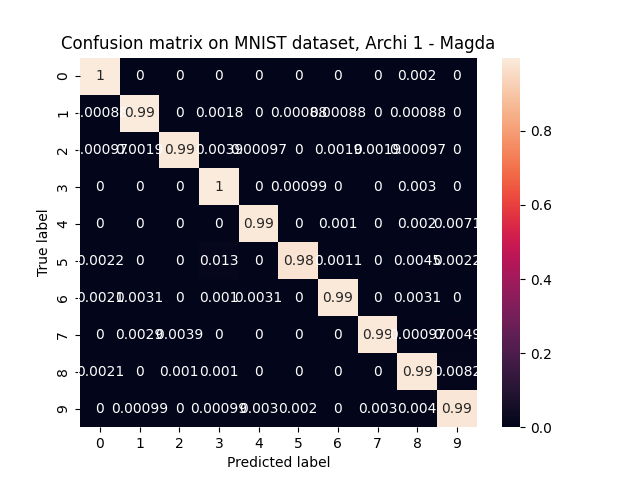
\includegraphics[width=\linewidth]{img/magda/MNIST_large_matrix}
        \caption{Macierz pomyłek}
    \end{subfigure}
    \caption{Wyniki dla 1 architektury (Train acc: 0.988; Test acc: 0.984)}
    \label{fig:exp1_magda_mnist}
\end{figure}


\subsection*{Druga architektura, prowadząca do ekstrakcji 2 cech}
Składa się z czterech warstw splotowych. Liczba filtrów w tych warstwach jest hierarchicznie zwiększana (32,64,128) kończąc na 2.
Po każdej warstwie splotowej następuje normalizacja wsadowa (BatchNorm2d), funkcja aktywacji ReLU i redukcja wymiarowości poprzez użycie operacji MaxPool2d, z wyjątkiem ostatniej warstwy, gdzie ta operacja nie jest już potrzebna.
Taka konfiguracja została zaprojektowana w celu stopniowego wyodrębniania coraz bardziej skomplikowanych cech z obrazów MNIST.
Pierwsze warstwy koncentrują się na wykrywaniu podstawowych cech, takich jak krawędzie i rogi, dzięki mniejszej liczbie filtrów.
Następnie, w kolejnych warstwach, liczba filtrów jest stopniowo zwiększana.
Operacje normalizacji wsadowej pomagają w stabilizacji uczenia poprzez zapewnienie jednolitego zakresu wartości na wyjściu z każdej warstwy, co może przyspieszyć proces uczenia oraz poprawić ogólną wydajność sieci.
Funkcja aktywacji ReLU została wybrana z powodu jej skuteczności w eliminowaniu zjawiska zanikającego gradientu i aktywowania jedynie istotnych cech.

Rezultaty tej metody zostały przedstawione poniżej na rys. ~\ref{fig:exp1_magda_mnist2}.

\pgfplotstableread[col sep=comma]{data/magda/mnist/small.csv}\MagdaMnistSmall{}

\begin{figure}[H]\centering
    \begin{subfigure}[b]{.55\textwidth}
        \plotAccuraciesFromLoggedMetrics{\MagdaMnistSmall}
        \caption{Wykres zmian accuracy}
    \end{subfigure}
    \begin{subfigure}[b]{.34\textwidth}
        \centering
        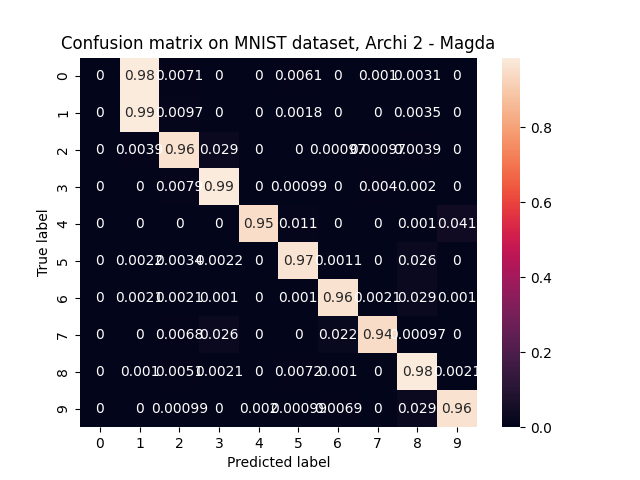
\includegraphics[width=\linewidth]{img/magda/MNIST_small_matrix}
        \caption{Macierz pomyłek}
    \end{subfigure}
    \caption{Wyniki dla 2 architektury (Train acc: 0.871; Test acc: 0.869)}\label{fig:exp1_magda_mnist2}
\end{figure}

\begin{wrapfigure}[1]{r}{0.4\textwidth}
    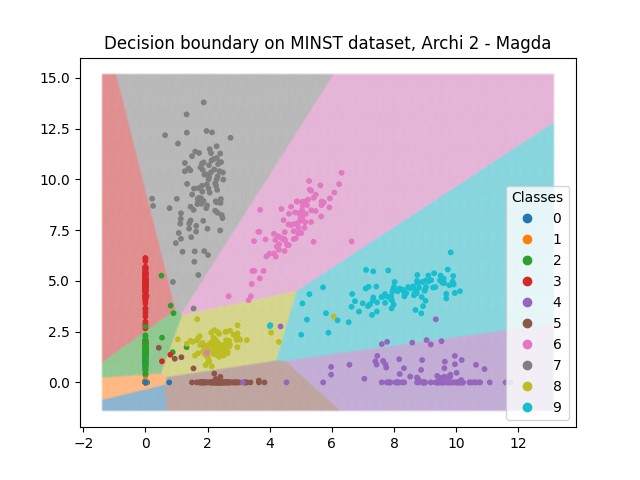
\includegraphics[width=\linewidth]{img/magda/MNIST_small_decision}
    \caption{Granica decyzyjna dla arch.~2}\label{fig:img/magda/MNIST_small_decision}
\end{wrapfigure}

Ekstraktor cech składa się z następujących warstw:

\tiny
\begin{verbatim}
(feature_extractor): Sequential(
    (0): Conv2d(1, 32, kernel_size=(3, 3), stride=(1, 1), padding=(1, 1))
    (1): BatchNorm2d(32)
    (2): ReLU()
    (3): MaxPool2d(kernel_size=2, stride=2)  # 32x28x28 -> 32x14x14

    (4): Conv2d(32, 64, kernel_size=(3, 3), stride=(1, 1), padding=(1, 1))
    (5): BatchNorm2d(64)
    (6): ReLU()
    (7): MaxPool2d(kernel_size=2, stride=2)

    (8): Conv2d(64, 128, kernel_size=(3, 3), stride=(1, 1), padding=(1, 1))
    (9): BatchNorm2d(128)
    (10): ReLU()
    (11): MaxPool2d(kernel_size=2, stride=2)

    (12): Conv2d(128, 2, kernel_size=(3, 3))
    (13): BatchNorm2d(2)
    (14): ReLU()
    (15): Flatten(start_dim=1)
)
(classifier): Sequential(
    (0): Linear(in_features=2, out_features=5, bias=True)
    (1): ReLU()
    (2): Linear(in_features=5, out_features=10, bias=True)
)
\end{verbatim}
\normalsize




\pagebreak
\section{Eksperyment 1: Architektury sieci splotowej dla CIFAR10 (Jakub Pawlak)}\label{sec:ex1-pawlak_cifar}

\subsection*{Pierwsza architektura}

\pgfplotstableread[col sep=comma]{data/kuba/cifar/large.csv}\kubaCifarLarge{}

Obrazy w zbiorze CIFAR10 są dużo bardziej złożone niż cyfry ze zbioru MNIST\@.
Przede wszystkim zawierają 3 kanały, a dodatkowo przedstawiają obiekty bardziej skomplikowane niż kształty cyfr.

Taka charakterystyka zbioru warunkuje zastosowanie głębszych sieci, zdolnych do ekstrakcji bardziej złożonych cech.

Głębsze architektury sieci skutkują większą ilością parametrów, a co za tym idzie, wolniejszym procesem uczenia.
W celu przyspieszenia uczenia, zdecydowano się na normalizację danych za pomocą warstw BatchNorm2d.

Ponadto, postanowiono poczynić eksperyment z połączeniami resztkowymi, inspirowanymi sieciami ResNet.

Ekstraktor cech składa się z 3 głównych etapów: \texttt{step\_1}, \texttt{step\_2}, \texttt{step\_3}.
Zawierają one warstwy splotowe, normalizacyjne, nieliniowe funckje aktywacji, jak również max pooling.
Zadaniem tych etapów jest zmniejszenie rozmiarów obrazu jak i ilości kanałów
(za wyjątkiem etapu \texttt{step\_1}, który zwiększa ilość kanałów, w celu ekstrakcji jak największej ilości cech w początkowej fazie).

Dodatkowo, etapy główne są oddzielone dwoma modułami resztkowymi (\texttt{residual\_1} oraz \texttt{residual\_2}), które nie zmieniają wymiarów obrazu.
Wejście do kolejnych warstw głównych stanowi suma wyjść z poprzedniej warstwy resztkowej oraz głównej.

Dzięki temu sieć staje się bardziej elastyczna --- jeśli warstwy splotowe nie są konieczne, sieć może wyuczyć się w ten sposób, aby wyjście z warstwy resztkowej było równe 0.
W ten sposób do następnego modułu głównego zostanie przekazane po prostu wyjście z poprzedniego modułu głównego, efektywnie ``pomijając'' moduł resztkowy.

\begin{figure}[H]\centering
    \begin{subfigure}[t]{.55\textwidth}
        \plotAccuraciesFromLoggedMetrics{\kubaCifarLarge}
        \caption{Wykres zmian accuracy}
    \end{subfigure}
    \hspace{2em}
    \begin{subfigure}[t]{.34\textwidth}
        \centering
        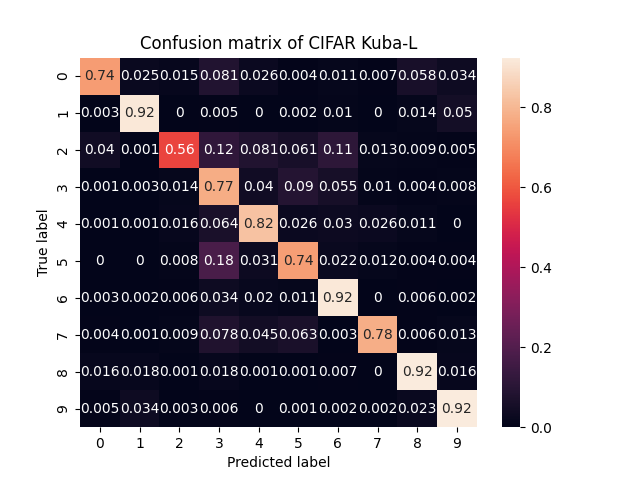
\includegraphics[width=\linewidth]{img/kuba/cifar/large_cm.png}
        \caption{Macierz pomyłek}
    \end{subfigure}
    \caption{Wyniki dla 1 architektury (Train acc: 0.931; Test acc: 0.810)}
    \label{fig:exp1_kuba_cifar}
\end{figure}


\subsection*{Druga architektura prowadząca do ekstrakcji 2 cech}

\pgfplotstableread[col sep=comma]{data/kuba/cifar/smol.csv}\kubaCifarSmol{}

\begin{figure}[H]\centering
    \begin{subfigure}[t]{.55\textwidth}
        \plotAccuraciesFromLoggedMetrics{\kubaCifarSmol}
        \caption{Wykres zmian accuracy}
    \end{subfigure}
    \hspace{2em}
    \begin{subfigure}[t]{.34\textwidth}
        \centering
        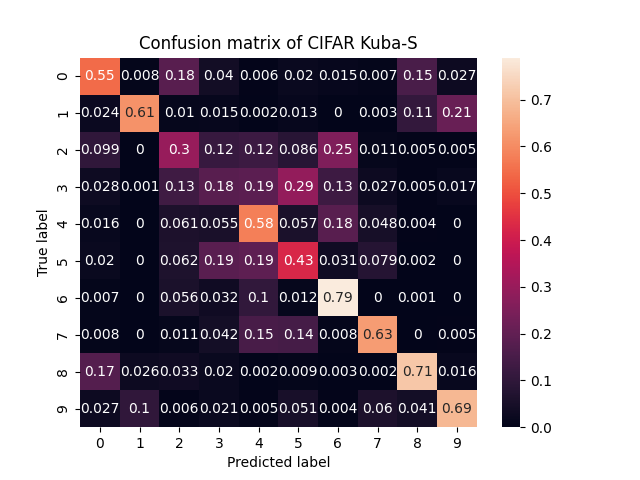
\includegraphics[width=\linewidth]{img/kuba/cifar/smol_cm.png}
        \caption{Macierz pomyłek}
    \end{subfigure}
    \caption{Wyniki dla 2 architektury (Train acc: 0.607; Test acc: 0.547)}
    \label{fig:exp1_kuba_cifar2}
\end{figure}


\begin{wrapfigure}[7]{r}{0.4\textwidth}
    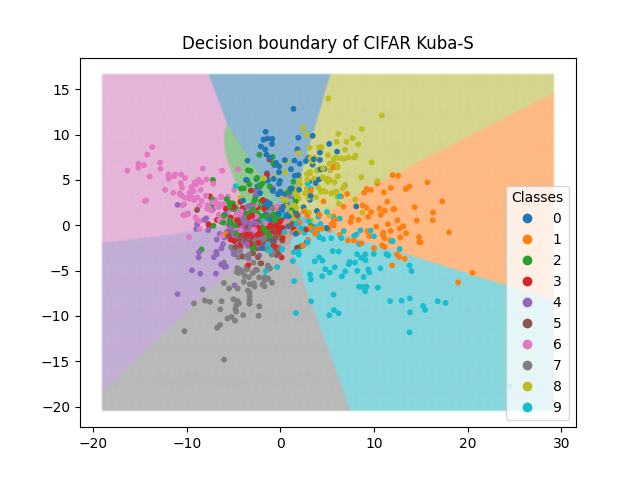
\includegraphics[width=\linewidth]{img/kuba/cifar/smol_db.png}
    \caption{Granica decyzyjna dla arch.~2}\label{fig:kuba/cifar/smol/decision_boundary}
\end{wrapfigure}

Druga architektura, podobnie jak przy zbiorze MNIST, dokonuje ekstrakcji cech do 2-elementowego wektora.
Z uwagi na niską rozdzielczość obrazków zdecydowano się użyć niewielkiego rozmiaru jądra w warstwach splotowych.
Podobnie jak w poprzednim modelu, dla przyspieszenia uczenia użyto warstw BatchNorm2d.
Standardowo, w celu zmniejszenia rozmiaru obrazów, a co za tym idzie ilości parametrów, użyte są warswty max pooling.
Na końcu ekstraktora cech dane zostają spłasczone do 2-elementowego wektora.

Klasyfikator standardowo składa się z 2 w pełni połączonych warstw.

\tiny
\begin{verbatim}
(feature_extractor): Sequential(
    (0): Conv2d(3, 64, kernel_size=(3, 3), stride=(1, 1), padding=(1, 1))
    (1): BatchNorm2d(64, eps=1e-05, momentum=0.1, affine=True, track_running_stats=True)
    (2): ReLU()
    (3): MaxPool2d(kernel_size=2, stride=2, padding=0, dilation=1, ceil_mode=False)
    (4): Conv2d(64, 32, kernel_size=(3, 3), stride=(1, 1), padding=(1, 1))
    (5): BatchNorm2d(32, eps=1e-05, momentum=0.1, affine=True, track_running_stats=True)
    (6): ReLU()
    (7): MaxPool2d(kernel_size=2, stride=2, padding=0, dilation=1, ceil_mode=False)
    (8): Conv2d(32, 8, kernel_size=(3, 3), stride=(1, 1), padding=(1, 1))
    (9): ReLU()
    (10): MaxPool2d(kernel_size=2, stride=2, padding=0, dilation=1, ceil_mode=False)
    (11): Conv2d(8, 2, kernel_size=(4, 4), stride=(1, 1))
    (12): Flatten(start_dim=1, end_dim=-1)
)
(classifier): Sequential(
    (0): Linear(in_features=2, out_features=16, bias=True)
    (1): ReLU()
    (2): Linear(in_features=16, out_features=10, bias=True)
)
\end{verbatim}
\normalsize

\pagebreak
\section{Eksperyment 1: Architektury sieci splotowej dla CIFAR10 (Magdalena Pakuła)}\label{sec:ex1-pakula_cifar}

\subsection*{Pierwsza architektura}
Składa się z trzech warstw splotowych, gdzie każda z nich wykorzystuje coraz większą liczbę filtrów o rozmiarze $3 \times 3$.
Pierwsza warstwa splotowa zawiera 32 filtry, stosuje funkcję aktywacji ReLU oraz warstwę Dropout z współczynnikiem 0.2, która losowo wyłącza część neuronów, zapobiegając nadmiernemu dopasowaniu.
Następnie warstwa MaxPooling zmniejsza rozmiar przestrzenny danych o połowę.
Druga warstwa splotowa składa się z 64 filtrów, ponownie stosuje ReLU oraz Dropout z współczynnikiem 0.3, a także warstwę MaxPooling, która zmniejsza rozmiar przestrzenny danych do $8 \times 8$.
Trzecia warstwa splotowa zawiera 128 filtrów, stosuje ReLU, Dropout z współczynnikiem 0.4 oraz MaxPooling, zmniejszając rozmiar przestrzenny danych do $4 \times 4$.
Dane są następnie spłaszczone do jednowymiarowego tensora za pomocą warstwy Flatten, umożliwiając przekazanie ich do warstw w pełni połączonych w celu klasyfikacji.
Klasyfikator składa się z dwóch warstw w pełni połączonych, gdzie pierwsza redukuje rozmiar cech do 128, stosując funkcję ReLU oraz Dropout z współczynnikiem 0.5, a druga warstwa klasyfikuje dane do liczby klas.
Ta architektura została zoptymalizowana w celu efektywnego wyodrębniania cech z obrazów o niskiej rozdzielczości, takich jak te występujące w zbiorze CIFAR\@.
Większa liczba warstw splotowych oraz zwiększenie liczby filtrów w każdej warstwie pozwalają na lepsze modelowanie danych, jednak możemy też zauważyć dosyć niskie train accuracy ze względu na ilość użyć funkcji Dropout.
Rezultaty tej metody zostały przedstawione na rys.~\ref{fig:exp1_magda_cifar}.

\pgfplotstableread[col sep=comma]{data/magda/cifar/large.csv}\MagdaCifarLarge{}

\begin{figure}[H]\centering
    \begin{subfigure}[b]{.55\textwidth}
        \plotAccuraciesFromLoggedMetrics{\MagdaCifarLarge}
        \caption{Wykres zmian accuracy}
    \end{subfigure}
    \begin{subfigure}[b]{.34\textwidth}
        \centering
        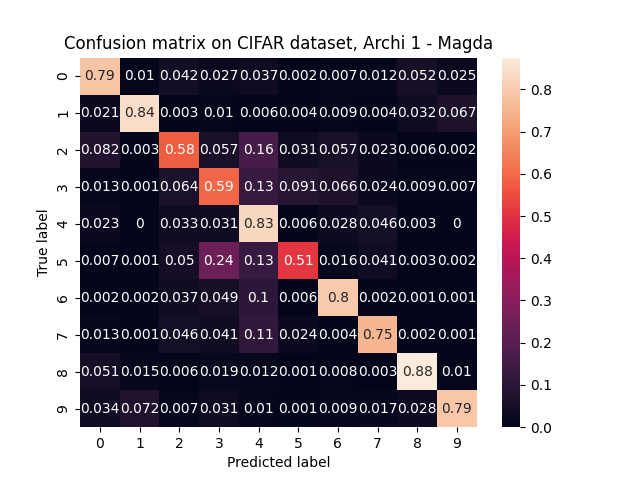
\includegraphics[width=\linewidth]{img/magda/CIFAR_large_matrix}
        \caption{Macierz pomyłek}
    \end{subfigure}
    \caption{Wyniki dla 1 architektury (Train acc: 0.623; Test acc: 0.679)}\label{fig:exp1_magda_cifar}
\end{figure}


\subsection*{Druga architektura prowadząca do ekstrakcji 2 cech}


\pgfplotstableread[col sep=comma]{data/magda/cifar/small.csv}\MagdaCifarSmall{}

\begin{figure}[H]\centering
    \begin{subfigure}[b]{.55\textwidth}
        \plotAccuraciesFromLoggedMetrics{\MagdaCifarSmall}
        \caption{Wykres zmian accuracy}
    \end{subfigure}
    \begin{subfigure}[b]{.34\textwidth}
        \centering
        \includegraphics[width=\linewidth]{img/magda/Cifar_small_matrix}
        \caption{Macierz pomyłek}
    \end{subfigure}
    \caption{Wyniki dla 2 architektury (Train acc: 0.539; Test acc: 0.573)}\label{fig:exp1_magda_cifar2}
\end{figure}

\begin{wrapfigure}[10]{r}{0.4\textwidth}
    \includegraphics[width=\linewidth]{img/magda/Cifar_small_decision}
    \caption{Granica decyzyjna dla arch.~2}\label{fig:img/magda/Cifar_small_decision}
\end{wrapfigure}

Składa się z 4 warstw splotowych z 32, 64 i 128 filtrami, które pozwalają na stopniowe wyodrębnianie coraz bardziej złożonych cech z danych wejściowych.
Następie użycie BatchNorm2d stabilizuje proces treningu i pozwala na szybsze uczenie się modelu, a funkcja aktywacji ReLU wprowadza nieliniowość.
Następnie jest wartswa MaxPooling redukująca rozmiar danych.
Ostatnia warstwa splotowa prowadzi do 2 filtrów.
Na końcu dodana jest Funkcja aktywacji ReLU\@.
Klasyfikator składa się z trzech warstw w pełni połączonych, które stopniowo redukują rozmiar cech i umożliwiają klasyfikację danych do odpowiedniej liczby klas.
Dropout (0.3) w pierwszej warstwie w pełni połączonej zapobiega nadmiernemu dopasowaniu modelu poprzez losowe wyłączanie neuronów podczas treningu.
Możemy dostrzec różnicę w klasyfikacji modelu, a użyciem funkcji Dropout w obu architekturach.

Rezultaty przedstawione są na rys.~\ref{fig:exp1_magda_cifar2}.

\tiny
\begin{verbatim}
(feature_extractor): Sequential(
    (0): Conv2d(3, 32, kernel_size=(3, 3), stride=(1, 1), padding=(1, 1))
    (1): BatchNorm2d(32)
    (2): ReLU()
    (3): MaxPool2d(kernel_size=2, stride=2)

    (4): Conv2d(32, 64, kernel_size=(3, 3), stride=(1, 1), padding=(1, 1))
    (5): BatchNorm2d(64)
    (6): ReLU()
    (7): MaxPool2d(kernel_size=2, stride=2)

    (8): Conv2d(64, 128, kernel_size=(3, 3), stride=(1, 1), padding=(1, 1))
    (9): BatchNorm2d(128)
    (10): ReLU()
    (11): MaxPool2d(kernel_size=2, stride=2)

    (12): Conv2d(128, 2, kernel_size=(4, 4))
    (13): ReLU()
    (14): Flatten(start_dim=1)
)
(classifier): Sequential(
    (0): Linear(in_features=2, out_features=128, bias=True)
    (1): ReLU()
    (2): Dropout(p=0.3)
    (3): Linear(in_features=128, out_features=64, bias=True)
    (4): ReLU()
    (5): Linear(in_features=64, out_features=num_classes, bias=True)
)
\end{verbatim}
\normalsize



\pagebreak
\section{Eksperyment 2: Wyniki dla MNIST}\label{sec:ex2_mnist}

\subsection*{Augmentacje}

\begin{multicols}{2}
    \paragraph{Jakub Pawlak}
    \small
    \begin{verbatim}
v2.RandomAffine(degrees=10, scale=(0.6, 1.5), shear=20)
    \end{verbatim}
    \normalsize
    Użyta transformacja łączy w sobie 3 różne techniki --- obrót, skalowanie i pochylenie.
    Cyfry mogą być obrócone o kąt pomiędzy $-10\degree$ a $10\degree$.
    Ma to na celu wytrenowanie modelu w rozpoznawaniu cyfr, nawet jeśli nie będą idealnie proste (nawet cyfra 1 na poniższym rysunku nie jest w oryginalnym zbiorze prosta).
    Kąt obrotu został ograniczony na tyle, żeby uzyskane w ten sposób obrazy wciąż przedstawiały odpowiednie cyfry (obraz cyfry 4 obrócona o 10\textdegree{} wciąż przedstawia cyfrę 4, jednak ten sam obraz obrócony o 180\textdegree{} nie przedstawiałby żadnej cyfry).
    Skalowanie ma na celu wprowadzenie do zbioru cyfr o różnym rozmiarze, w nadziei, że sprawi to, że sieć wyuczy się rozpoznawania cyfr po kształcie, a nie po lokalizacji konkretnych pikseli.
    Obrazy są również pochylone (\emph{ang. shear}) ponieważ, pisząc odręcznie, wiele ludzi pisze właśnie w sposób pochyły.
    \newcolumn{}
    \paragraph{Magdalena Pakuła}
    \small
    \begin{verbatim}
v2.ElasticTransform(alpha=50.0, sigma=5.0)
    \end{verbatim}
    \normalsize
    Użyta transformacja symuluje lekkie wypaczenie lub rozciągnięcie odręcznie zapisanych cyfr, naśladując naturalne różnice w sposobie pisania.
    Obrazy są zniekształcone w sposób elastyczny z parametrem $\alpha=50.0$ i odchyleniem standardowym $\sigma=5.0$.
    Ma to znaczenie dla zbioru MNIST, ponieważ pismo odręczne w świecie rzeczywistym może być nieco zniekształcone w porównaniu z cyfrą idealnie wyśrodkowaną i proporcjonalną.
    Dzięki temu transformacja ta pozwala modelowi lepiej radzić sobie z różnicami w naturalnym piśmie odręcznym, poprawiając jego zdolność do generalizacji.
    Przykładowo, cyfry mogą być delikatnie rozciągnięte lub skręcone, co wprowadza do zbioru bardziej realistyczne wariacje.
\end{multicols}

\begin{figure}[H]\centering
    \begin{subfigure}[t]{.45\textwidth}
        \centering
        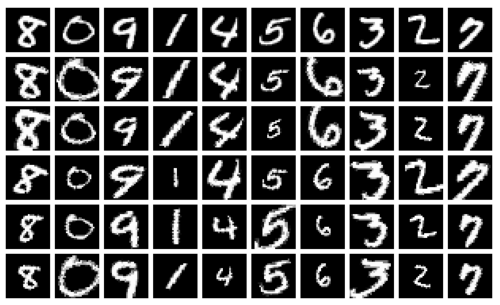
\includegraphics[width=.7\linewidth]{img/kuba/mnist/augmentations.png}
        \caption{Jakub Pawlak}
    \end{subfigure}
    \begin{subfigure}[t]{.45\textwidth}
        \centering
        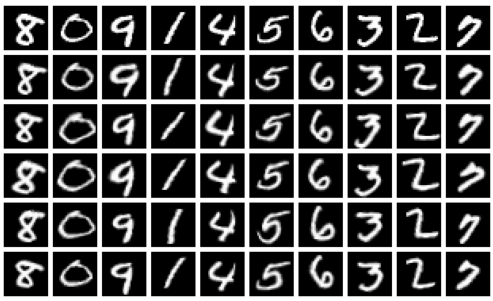
\includegraphics[width=0.7\linewidth]{img/magda/augmented_MNIST}
        \caption{Magdalena Pakuła}
    \end{subfigure}
    \caption{Augmentacje dla zbioru MNIST (górny wiersz zawiera oryginalne obrazki)}
\end{figure}


\subsection*{Najlepsza architektura}

Architektura Kuba

\begin{table}[H]\centering
    \begin{tabular}{cccccc}
        \toprule
                         & \multicolumn{5}{c}{Ilość obrazów}                                                                                   \\ \cmidrule{2-6}
        Augmentacja      & 10                                & 100               & 200                & 1000              & 10\,000            \\ \midrule
        Jakub Pawlak     & $0.100 \pm 0.001 $                & $0.541 \pm 0.161$ & $0.795 \pm 0.042 $ & $0.921 \pm 0.024$ & $0.942 \pm 0.008 $ \\
        Magdalena Pakuła & $0.100 \pm 0.000 $                & $0.651 \pm 0.051$ & $0.811 \pm 0.033$ & $0.931 \pm 0.019$ & $0.948 \pm 0.008$ \\
        Brak             &                                 & $0.100 \pm 0.000$ & $0.100 \pm 0.000$  & $0.638 \pm 0.145$ & $0.931 \pm 0.016$  \\
        \bottomrule
    \end{tabular}
    \caption{Wyniki dla 1 architektury na zbiorze MNIST z augmentacją (accuracy z 10 prób w formie $\mu \pm \sigma$)}
\end{table}

\subsection*{Najlepsza architektura prowadząca do ekstrakcji 2 cech}

Architektura Magda

\begin{table}[H]\centering
    \begin{tabular}{cccccc}
        \toprule
                         & \multicolumn{5}{c}{Ilość obrazów}                                                                                   \\ \cmidrule{2-6}
        Augmentacja      & 10                                & 100                & 200                & 1000              & 10\,000           \\ \midrule
        Jakub Pawlak     & $0.106 \pm 0.031 $                & $0.130 \pm 0.037 $ & $0.385 \pm 0.037 $ & $0.530 \pm 0.045$ & $0.671 \pm 0.020$ \\
        Magdalena Pakuła & $0.134 \pm 0.041 $                & $0.164 \pm 0.052$  & $0.375 \pm 0.054 $ & $0.533 \pm 0.039$ & $0.707 \pm 0.038$                     \\
        Brak             &                                 & $0.152 \pm 0.040$  & $0.142 \pm 0.033$  & $0.147 \pm 0.020$ & $0.564 \pm 0.011$ \\
        \bottomrule
    \end{tabular}
    \caption{Wyniki dla 2 architektury na zbiorze MNIST z augmentacją (accuracy z 10 prób w formie $\mu \pm \sigma$)}
    \label{tab:Wyniki_small_MNIST_tabela}
\end{table}

\pagebreak
\section{Eksperyment 2: Wyniki dla CIFAR10}\label{sec:ex2_cifar}

\subsection*{Augmentacje}

\begin{multicols}{2}
    \paragraph{Jakub Pawlak}
    \scriptsize
    \begin{verbatim}
v2.RandomAffine(degrees=15, translate=(0.1, 0.1), scale=(1, 1.2), shear=10),
v2.Resize((36, 36)),
v2.RandomCrop((32, 32)),
v2.ColorJitter(brightness=0.2, hue=0.05, saturation=0.1)
    \end{verbatim}
    \normalsize
    W tym przypadku, podobnie jak dla poprzedniego zbioru danych, użyto transformacji \emph{RandomAffine}.
    Jednakże, w wyniku tej transformacji mogą pojawić się na obrazie nowe piksele, mające kolor czarny.
    O ile w przypadku zbioru MNIST nie było to problemem, ponieważ tamte obrazy miały czarne tło, o tyle w przypadku zbioru CIFAR, tła są kolorowe.
    Duże strefy czerni wprowadzone w wyniku augmentacji nie są więc czymś normalnie występującym w zbiorze, mogłyby zatem wypaczać uczenie.
    W celu niwelacji tego problemu, zastosowano zwiększenie rozmiaru obrazu do $36\times36$, a następnie przycięcie go do oryginalnego rozmiaru, w nadziei, że w ten sposób czarne artefakty na krawędziach zostaną w większości ``wycięte''.
    Na końcu, ponieważ zbiór przedstawia kolorowe obrazy, zastosowano efekt \emph{ColorJitter} delikatnie zmieniający jasność, odcień i nasycenie.
    W ten sposób model nie powinien łączyć poszczególnych klas z bardzo konkretnymi barwami.
    \newcolumn{}
    \paragraph{Magdalena Pakuła}
    \scriptsize
    \begin{verbatim}
v2.RandomRotation(degrees=30),
v2.RandomErasing(p=0.5, scale=(0.02, 0.2), ratio=(0.3, 3.3), value='random'),
v2.RandomAffine(degrees=20, translate=(0.1, 0.1), scale=(0.8, 1.2), shear=15),
v2.ColorJitter(brightness=0.3, contrast=0.3, saturation=0.3, hue=0.1),
v2.GaussianBlur(kernel\_size=3)
\end{verbatim}
    \normalsize
    W tej technice losowo obracamy obrazy o maksymalnie 30 stopni, co pozwala na uczenie na różne orientacje obiektów w obrazach.
    Następnie, losowo zacieramy części obrazu z pewnym prawdopodobieństwem (0.5), co symuluje uszkodzenia obrazu lub brak danych.
    Użyta transformacja \emph{RandomAffine} łączy w sobie przesunięcie, skalowanie i skręcanie obrazu, z maksymalnym kątem obrotu 20 stopni, translacją do 10\%, skalowaniem od 80\% do 120\%, i pochyleniem do 15 stopni.
    Dodano również efekt \emph{ColorJitter}, który zmienia jasność, kontrast, nasycenie i barwę, co jest szczególnie istotne w przypadku kolorowych obrazów.
    Ostatecznie, rozmycie Gaussowskie o rozmiarze jądra 3 pomaga w redukcji szumów oraz zwiększa zdolność modelu do generalizacji poprzez usuwanie drobnych szczegółów, które mogą być przypadkowe lub nieistotne dla klasyfikacji.
\end{multicols}

\begin{figure}[H]\centering
    \begin{subfigure}[t]{.45\textwidth}
        \centering
        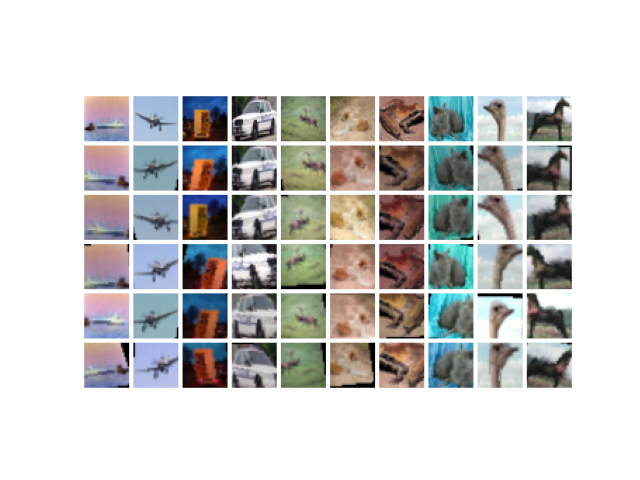
\includegraphics[width=.7\linewidth]{img/kuba/cifar/augmentations.png}
        \caption{Jakub Pawlak}
    \end{subfigure}
    \begin{subfigure}[t]{.45\textwidth}
        \centering
        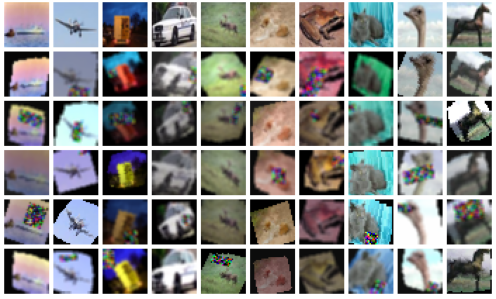
\includegraphics[width=.7\linewidth]{img/magda/augmented_CIFAR}
        \caption{Magdalena Pakuła}
    \end{subfigure}
    \caption{Augmentacje dla zbioru CIFAR10 (górny wiersz zawiera oryginalne obrazki)}
\end{figure}


\subsection*{Najlepsza architektura}

Architektura Kuba

\begin{table}[H]\centering
    \begin{tabular}{cccccc}
        \toprule
                         & \multicolumn{5}{c}{Ilość obrazów}                                                                                    \\ \cmidrule{2-6}
        Augmentacja      & 10                                & 100                & 200                & 1000              & 10\,000            \\ \midrule
        Jakub Pawlak     & $0.126 \pm 0.014 $                & $0.224 \pm 0.028 $ & $0.298 \pm 0.021 $ & $0.466 \pm 0.029$ & $0.656 \pm 0.009 $ \\
        Magdalena Pakuła & $0.151 \pm 0.016 $                &  $0.206 \pm 0.021$ & $0.263 \pm 0.013 $ & $0.412 \pm 0.038$  & $0.522 \pm 0.010$    \\
        Brak             &                                   & $0.142 \pm 0.025$  & $0.180 \pm 0.004$  & $0.294 \pm 0.025$ & $0.637 \pm 0.009$  \\
        \bottomrule
    \end{tabular}
    \caption{Wyniki dla 1 architektury na zbiorze CIFAR z augmentacją (accuracy z 10 prób w formie $\mu \pm \sigma$)}\label{tab:augmented_cifar_big}
\end{table}

\subsection*{Najelpsza architektura prowadząca do ekstrakcji 2 cech}

Arch. Magda

\begin{table}[H]\centering
    \begin{tabular}{cccccc}
        \toprule
                         & \multicolumn{5}{c}{Ilość obrazów}                                                                                    \\ \cmidrule{2-6}
        Augmentacja      & 10                                & 100                & 200                & 1000              & 10\,000            \\ \midrule
        Jakub Pawlak     & $0.100 \pm 0.001 $                & $ 0.100 \pm 0.000$ & $0.100 \pm 0.000 $ & $0.137 \pm 0.046$ & $0.184 \pm 0.084 $ \\
        Magdalena Pakuła & $0.099 \pm 0.004 $                & $0.100 \pm 0.000$ & $0.100 \pm 0.000 $ & $0.108 \pm 0.023$  & $0.197 \pm 0.053$   \\
        Brak             &                                   & $0.100 \pm 0.000$  & $0.100 \pm 0.000$  & $0.100 \pm 0.000$ & $0.123 \pm 0.046$  \\
        \bottomrule
    \end{tabular}
    \caption{Wyniki dla 2 architektury na zbiorze CIFAR z augmentacją (accuracy z 10 prób w formie $\mu \pm \sigma$)}\label{tab:augmented_cifar_small}
\end{table}

\pagebreak
\section{Analiza i wnioski}\label{sec:wyniki}
\subsection*{Porównanie architektur sieci splotowych}
W pierwszej architekturze dla zbioru MNIST wyniki zaprezentowane są bardzo podobne:
0.987 i 0.984 (patrz: rys.~\ref{fig:exp1_kuba_mnist} i rys.~\ref{fig:exp1_magda_mnist}).
Wynika to z faktu, że ten zbiór nie jest zbytnio skomplikowany i przy obu modelach można w sieci splotowej można otrzymać rewelacyjne wyniki.
Różnica w wyniku może wynikać z bardziej złożonego klasyfikatora z 3 warstwami liniowymi w lepszym modelu w porównanu z jedną warstwa liniową w gorszym.

W drugiej architekturze dla zbioru MNIST występuje podobna sytuacja, gdzie wyniki to odpowiednio 0.866 i 0.869 (rys.~\ref{fig:kuba/mnist/smol} i~\ref{fig:exp1_magda_mnist2}).
W tym wypadku modele na tym zbiorze działają podobnie.
Minimalna różnica może polegać na fakcie, iż drugi model ma większą liczbę kanałów w warstwach konwolucyjnych, co może pomóc w wydobyciu bardziej złożonych cech, jednak jest to jak widać różnica minimalna.
Zaskakującym może wydawać się fakt, iż model drugi uzyskuje lepszy wynik accuracy, pomimo, że jest całkowicie niezdolny do rozpoznania cyfry ``0''.

Można również zauważyć ``przycinanie'' ujemnych współrzędnych wynikające z użycia funkcji ReLU na wyjściu ekstraktora cech,
co bardzo dobrze widać na rys.~\ref{fig:img/magda/MNIST_small_decision}.
Aby uniknąć tego zjawiska, model znajdujący się na rys.~\ref{fig:kuba/cifar/smol/decision_boundary} nie zawiera funkcji ReLU na wyjściu ekstraktora cech.
Jednakże, w momencie pisania tychże wniosków, okazuje się, że nie była to zbyt mądra decyzja, ponieważ skutkuje to bezpośrednim sąsiedztwem dwóch warstw liniowych, co negatywnie wpływa na możliwości modelu.
Podobny problem zawiera również 2 architektura opisana w sekcji 3.

W pierwszej architekturze dla zbioru CIFAR zdecydowanie lepsze wyniki osiąga model pierszy ---
0.810 (rys.~\ref{fig:exp1_kuba_cifar}) kontra 0.679 (rys.~\ref{fig:exp1_magda_cifar}).
Pierwszy model ma bardziej złożoną architekturę, a decydującą różnicą jest użycie połączeń resztkowych (\emph{ang. residual connections}), które zwiększają elastyczność modelu.
Na wykresie accuracy na rys.~\ref{fig:exp1_magda_cifar}można również zauważyć, że accuracy na zbiorze treningowym jest niższe niż na testowym, co wynika ze zbyt dużej ilości warstw Dropout, na co należy uważać.

W drugiej architekturze dla zbioru CIFAR wyniki wyniosły odpowiednio 0.547 i 0.573 (patrz: rys.~\ref{fig:exp1_kuba_cifar2} i~\ref{fig:exp1_magda_cifar2}).
W tym wypadku modele osiągają podobne wyniki, jednak minimalna różnica może wynikać z faktu, iż drugi model jest bardziej zaawansowany --- posiada więcej warstw konwolucyjnych i wartsw Dropout, co wpływa na mniejszą zdolność do nauki skomplikowanych wzorów w zbiorze.
Warto zauważyć overfitting w późniejszych epochach dla modelu drugiego, który może wynikać z braku regularyzacji (np.
przez Dropout), przez co model nadmiernie dopasowuje sie do danych treningowych.

Różnice w wartości accuracy na zbiorze testowym na obu zbiorach danych wynikają ze złożoności i skomplikowania zbioru CIFAR nad dość prostym wizuzalnie zbiorem MNIST\@.
Niekiedy obrazki ze zbioru CIFAR mogą być trudno rozpoznawalne dla ludzkiego oka, a tym bardziej dla modelu.
Niemniej jednak, modele wykorzystane w eksperymentach poradziły sobie z zadaniem klasyfikacji zadowalająco.

\subsection*{Wpływ augmentacji danych}
Przy ocenie wpływu liczby danych treningowych, można wprost zauważyć, że większa liczba przykładów treningowych prowadzi do lepszych wyników.
Oba rodzaje augmentacji przyniosły poprawę wyników, jednakże zauważono, że augmentacja dla zbioru MNIST za pomocą \textit{ElsticTransform} osiągnęła lepsze wyniki w porównaniu do augmentacji za pomocą \textit{RandomAffine}.
Jest to prawdopodobnie spowodowane tym, że \textit{ElasticTransform} wprowadza bardziej losowe i skomplikowane transformacje, co może zwiększyć różnorodność danych treningowych i pomóc w lepszym uogólnieniu modelu oraz może lepiej radzić sobie z zastosowanymi deformacjami, co jest szczególnie przydatne w przypadku danych obrazowych.

W przypadku augmentacji na zbiorze CIFAR lepszą augmentacją okazała się ta zaproponowana przez pierwszą osobę, gdzie na 1000 przypadków test accuracy wynosiło w 1 architekturze 0.466 oraz 0.137 (w porównaniu z 0.412 i 0.108) tab. ~\ref{tab:augmented_cifar_big} i tab. ~\ref{tab:augmented_cifar_small}.
Jest to znów niewielka różnica, jednak wynika ona z faktu, iż pierwsza augmentacja stosuje mniej agresywne transformacje, które dodają różnorodność bez nadmiernego zniekształcania obrazów.
Augmentacje takie jak \textit{RandomHorizontalFlip} i drobne zmiany w jasności i odcieniu, pomagają modelowi lepiej generalizować, unikając nadmiernego dopasowania do specyficznych wzorców.
Druga augmentacja wprowadza bardziej agresywne zmiany, takie jak \textit{RandomRotation} i \textit{RandomErasing}, które w przypadku zbioru CIFAR o małej rozdzielczości prowadzą do utraty istotnych informacji a dodatkowo \textit{GaussianBlur} zmniejsza już niską wyrazistość kluczowych cech w obrazach, co utrudnia modelowi naukę.
Jednakże, model przy takich trudnych zmianach poradził sobie w porządku, a takie transformacje zostały zaproponowane w ramach testu i sprawdzenia jak zbiór poradziłby sobie z takimi zmianami.

Zauważyliśmy, że augmentacja danych na MNIST prowadzi do niewielkiego, ale zauważalnego wzrostu dokładności.
Ponieważ zestaw danych jest stosunkowo prosty i dobrze zdefiniowany, bazowy model sieci może osiągnąć wysoką dokładność nawet bez augmentacji.
Niemniej jednak, dodanie augmentacji może pomóc modelowi lepiej generalizować na niewielkie wariacje w danych, co prowadzi do poprawy wyników.

Co innego następuje w zbiorze CIFAR, który posiada bardziej złożone zestawy danych i ze względu na większą różnorodność i złożoność obrazów, augmentacja danych jest bardziej istotna.
Dobrze zdefiniowane augmentacje danych prowadzą do wzrostu dokładności modelu, jednak ze względu na tą złożoność danych, modele sieci mogą też być podatne na overfitting.
Zastosowanie augmentacji pomaga w zapobieganiu przetrenowaniu poprzez zwiększenie różnorodności danych treningowych, co z kolei pomaga modelowi lepiej generalizować na nowe, niewidoczne dane.

\end{document}